%-----------------------------------------------------------------------------------------------
\chapter{Marker-based Pose Estimation}\label{sect:marker_recognition}
%-----------------------------------------------------------------------------------------------

The main goal fo this work is to devise a fiducial marker and a method of estimating the camera pose based on it.
In the previous chapters the most of the building blocks used to achieve this were laid out.
The marker have been defined and the image processing algorithms used for measuring quad positions were explained.
In this chapter a solution will be given to the task of estimating the camera pose based on a single shot of the above described markers.

\begin{figure}[ht]
	\centering
	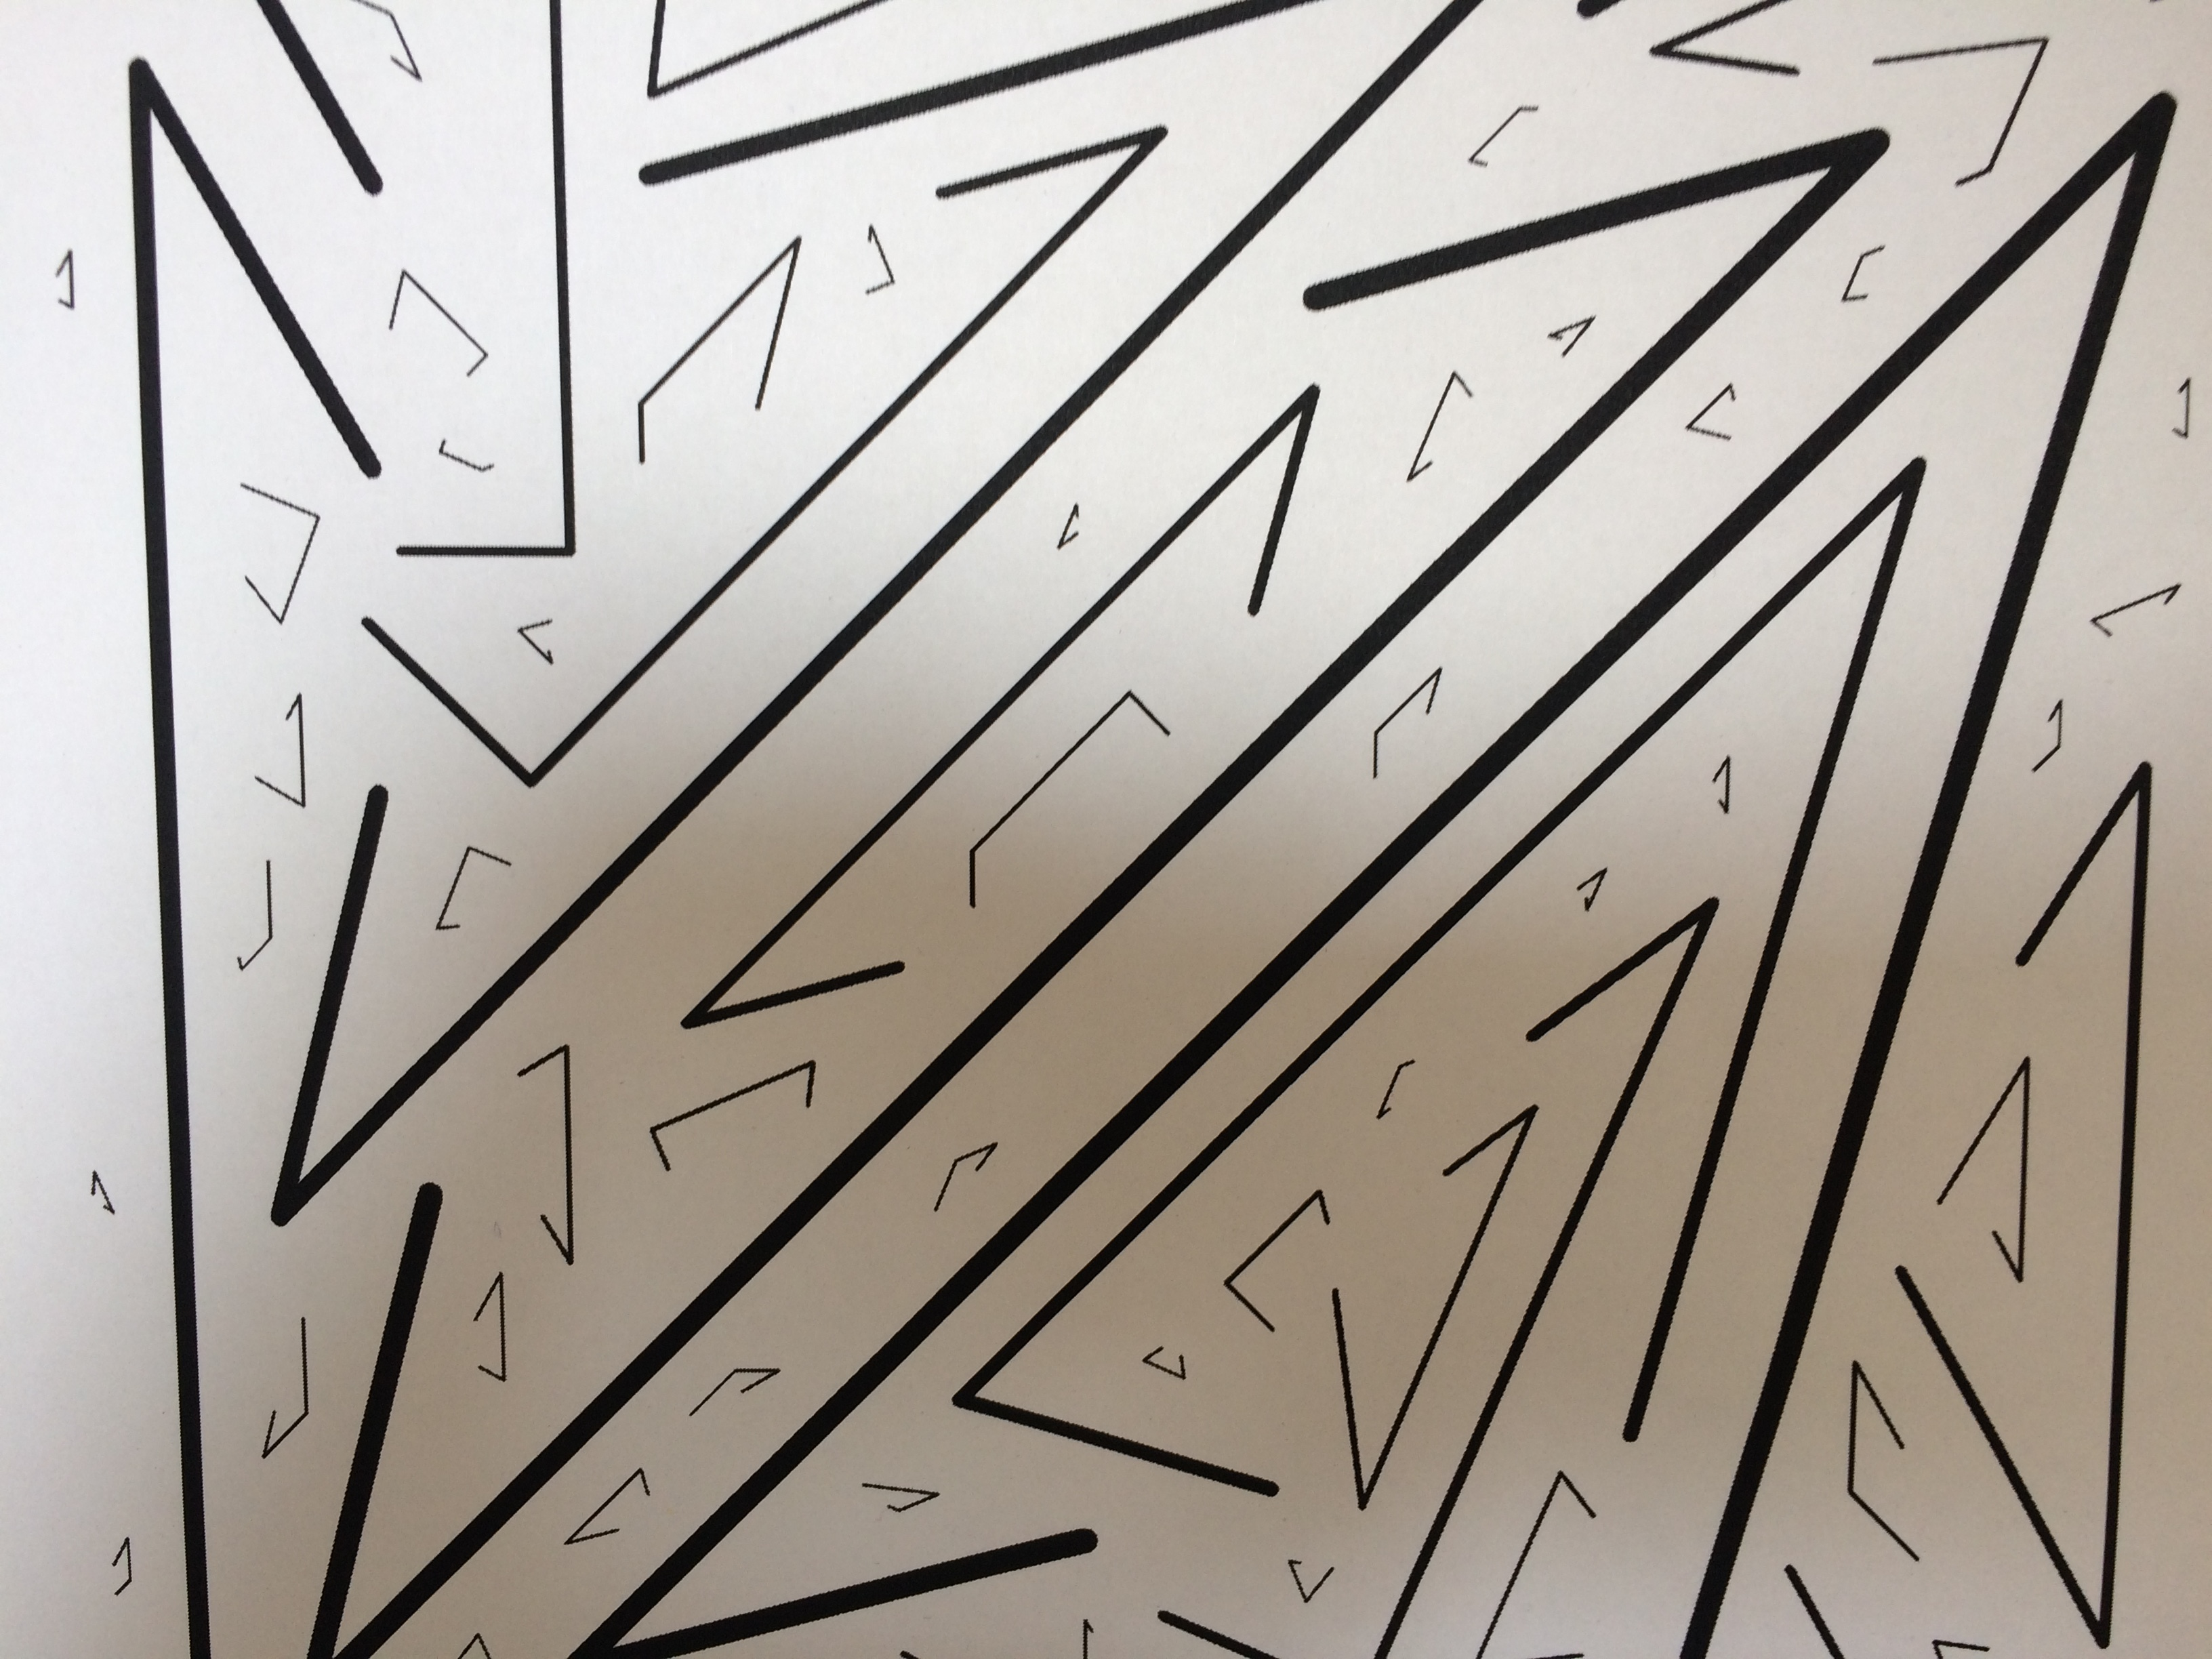
\includegraphics[width=0.9\textwidth]{figures/marker_full.JPG}
	\caption{Shot of a partially visible marker covering the whole field of vision}
	\label{fig:markerFull}
\end{figure}

As it's input, the algorithm will receive an image containing the marker (figure \figref{markerFull} shows an example).
The image does not have to be ideal.
Quite probably some of the marker's surroundings are also visible, or equally probably only a part of the marker is visible.
Using commercially available cameras the image almost certainly contains some level of noise.
The algorithm has to be prepared for handling these cases.
This is achieved by applying a range of preprocessing steps to the input image.

When the input image have been aptly conditioned, the regions containing quads have to be identified.
The previously described quad detection routines work on images containing a single quad\footnote{Although they could be implemented to handle whole markers at once}, so the input have to be segmented before quad detection.
These two steps (identifying quad-like regions and segmentation) are done in a single a step based on extracting blobs that meet certain criteria typical for quads.

The next step in the processing pipeline is running the quad detection algorithm on the previously selected segments.
It is executed for each quad-like blob, and the successfully identified quads are stored in a list for later processing.
If enough quads have been found, the pose can be calculated.

The last necessary step is to actually estimate the camera pose.
This is an iterative process, as the pairing of original and detected quads are not known prior to successfully approximating the viewpoint.
This algorithm was designed supposing the marker on the image is known and only the camera pose has to be calculated.
For the purposes of this project the assumptions is reasonable, as for now, no meta-information is coded into the markers.
Also, for the current stage a single point of reference for the pose is enough.

The above steps of the pose estimation algorithm are summarised in the following pseudo-code.
\begin{lstlisting}
estimate_pose(img, original_marker):
    img = prepare_img(img)
    quad_imgs = get_segments(img)
    quads = empty_list
    for quad_img in quad_imgs
        quad = detect_quad(quad_img)
        quads.append(quad)
    pose = find_pose(quads, orignal_marker) 
    return pose
\end{lstlisting}
The following sections will elaborate on each step of the process.
The quad detection algorithms were already covered, their explanation can be found in the relevant chapter.
The pose calculation from the corresponding point pairs will also not be covered, as the algorithm was described in chapter 1.

%-----------------------------------------------------------------------------------------------
\section{Preprocessing}
%-----------------------------------------------------------------------------------------------

The input of the preprocessing step is the raw image taken\footnote{In the development phase rendered pictures were used for better repeatability} by the observer.
The goal of this step is preparing the input image for the next phases (segmentation, filtering, quad detection) of processing visual data.
As mentioned in the introduction, the raw input image can have a variety of distortions.
Some of these are systematic and thus easy accounted for, others are random and their effects can only be dampened.
An example of the first one the barrel distortion caused by the camera lens, and of the latter is the \textit{salt and pepper} noise of the image.

The systematic errors are corrected by using a calibrated camera.
Camera calibration will not be covered in depth, as multiple well tried solutions exist for it.
In this project a calibration method provided by the OpenCV framework was used.
It uses a chessboard pattern as a calibration image to measure the intrinsic camera parameters.
The OpenCV framework uses \eqref{cameraMat} for a camera model.
\begin{equation}
	C_m = 
	\begin{bmatrix}
		f_x & 0   & c_x \\
		0   & f_y & c_y \\
		0   & 0   & 1
	\end{bmatrix}
	\label{eq:cameraMat}
\end{equation}
The parameters correspond to the usual notation:
\begin{itemize}
	\item $f_x, f_y$: Focal lengths of the camera in $x$ and $y$ direction
	\item $c_x, c_y$: The coordinates of the optical centre in the image
\end{itemize}
Based on the camera matrix, OpenCV can account for most of the radial and tangential distortion in the image.

The filtering of random noise from the image is a bigger issue, and no exact solution can be given for it.
There are many factors that can influence the quality of the image.
The lighting conditions, the shadows, the viewing angle, etc...
Not all of them can (reasonably) be accounted for.
However, to lessen their impact on the image, the following steps are taken.

First the photos are converted to binary format by applying a threshold.
The image is inverted in the process, because it makes more sense for the objects to be marked with non-zero elements than vice-versa.
The threshold's value is determined using Otsu's method, which maximises the inter-class variance of the clusters\footnote{Foreground and background}.
The implementation is provided by the OpenCV framework.

Afterwards, the binary image is conditioned with a \emph{close} morphology operator.
The closing removes the gaps from the large connected areas (possible quads) and removes the \emph{salt and pepper}-like noise.
In the current implementation the kernel size of the morphology operator is constant, however it could be beneficial to calculate it from the global or local image parameters\footnote{e.g. image size, area of the connected region, etc.}.

\begin{figure}[ht]
	\centering
	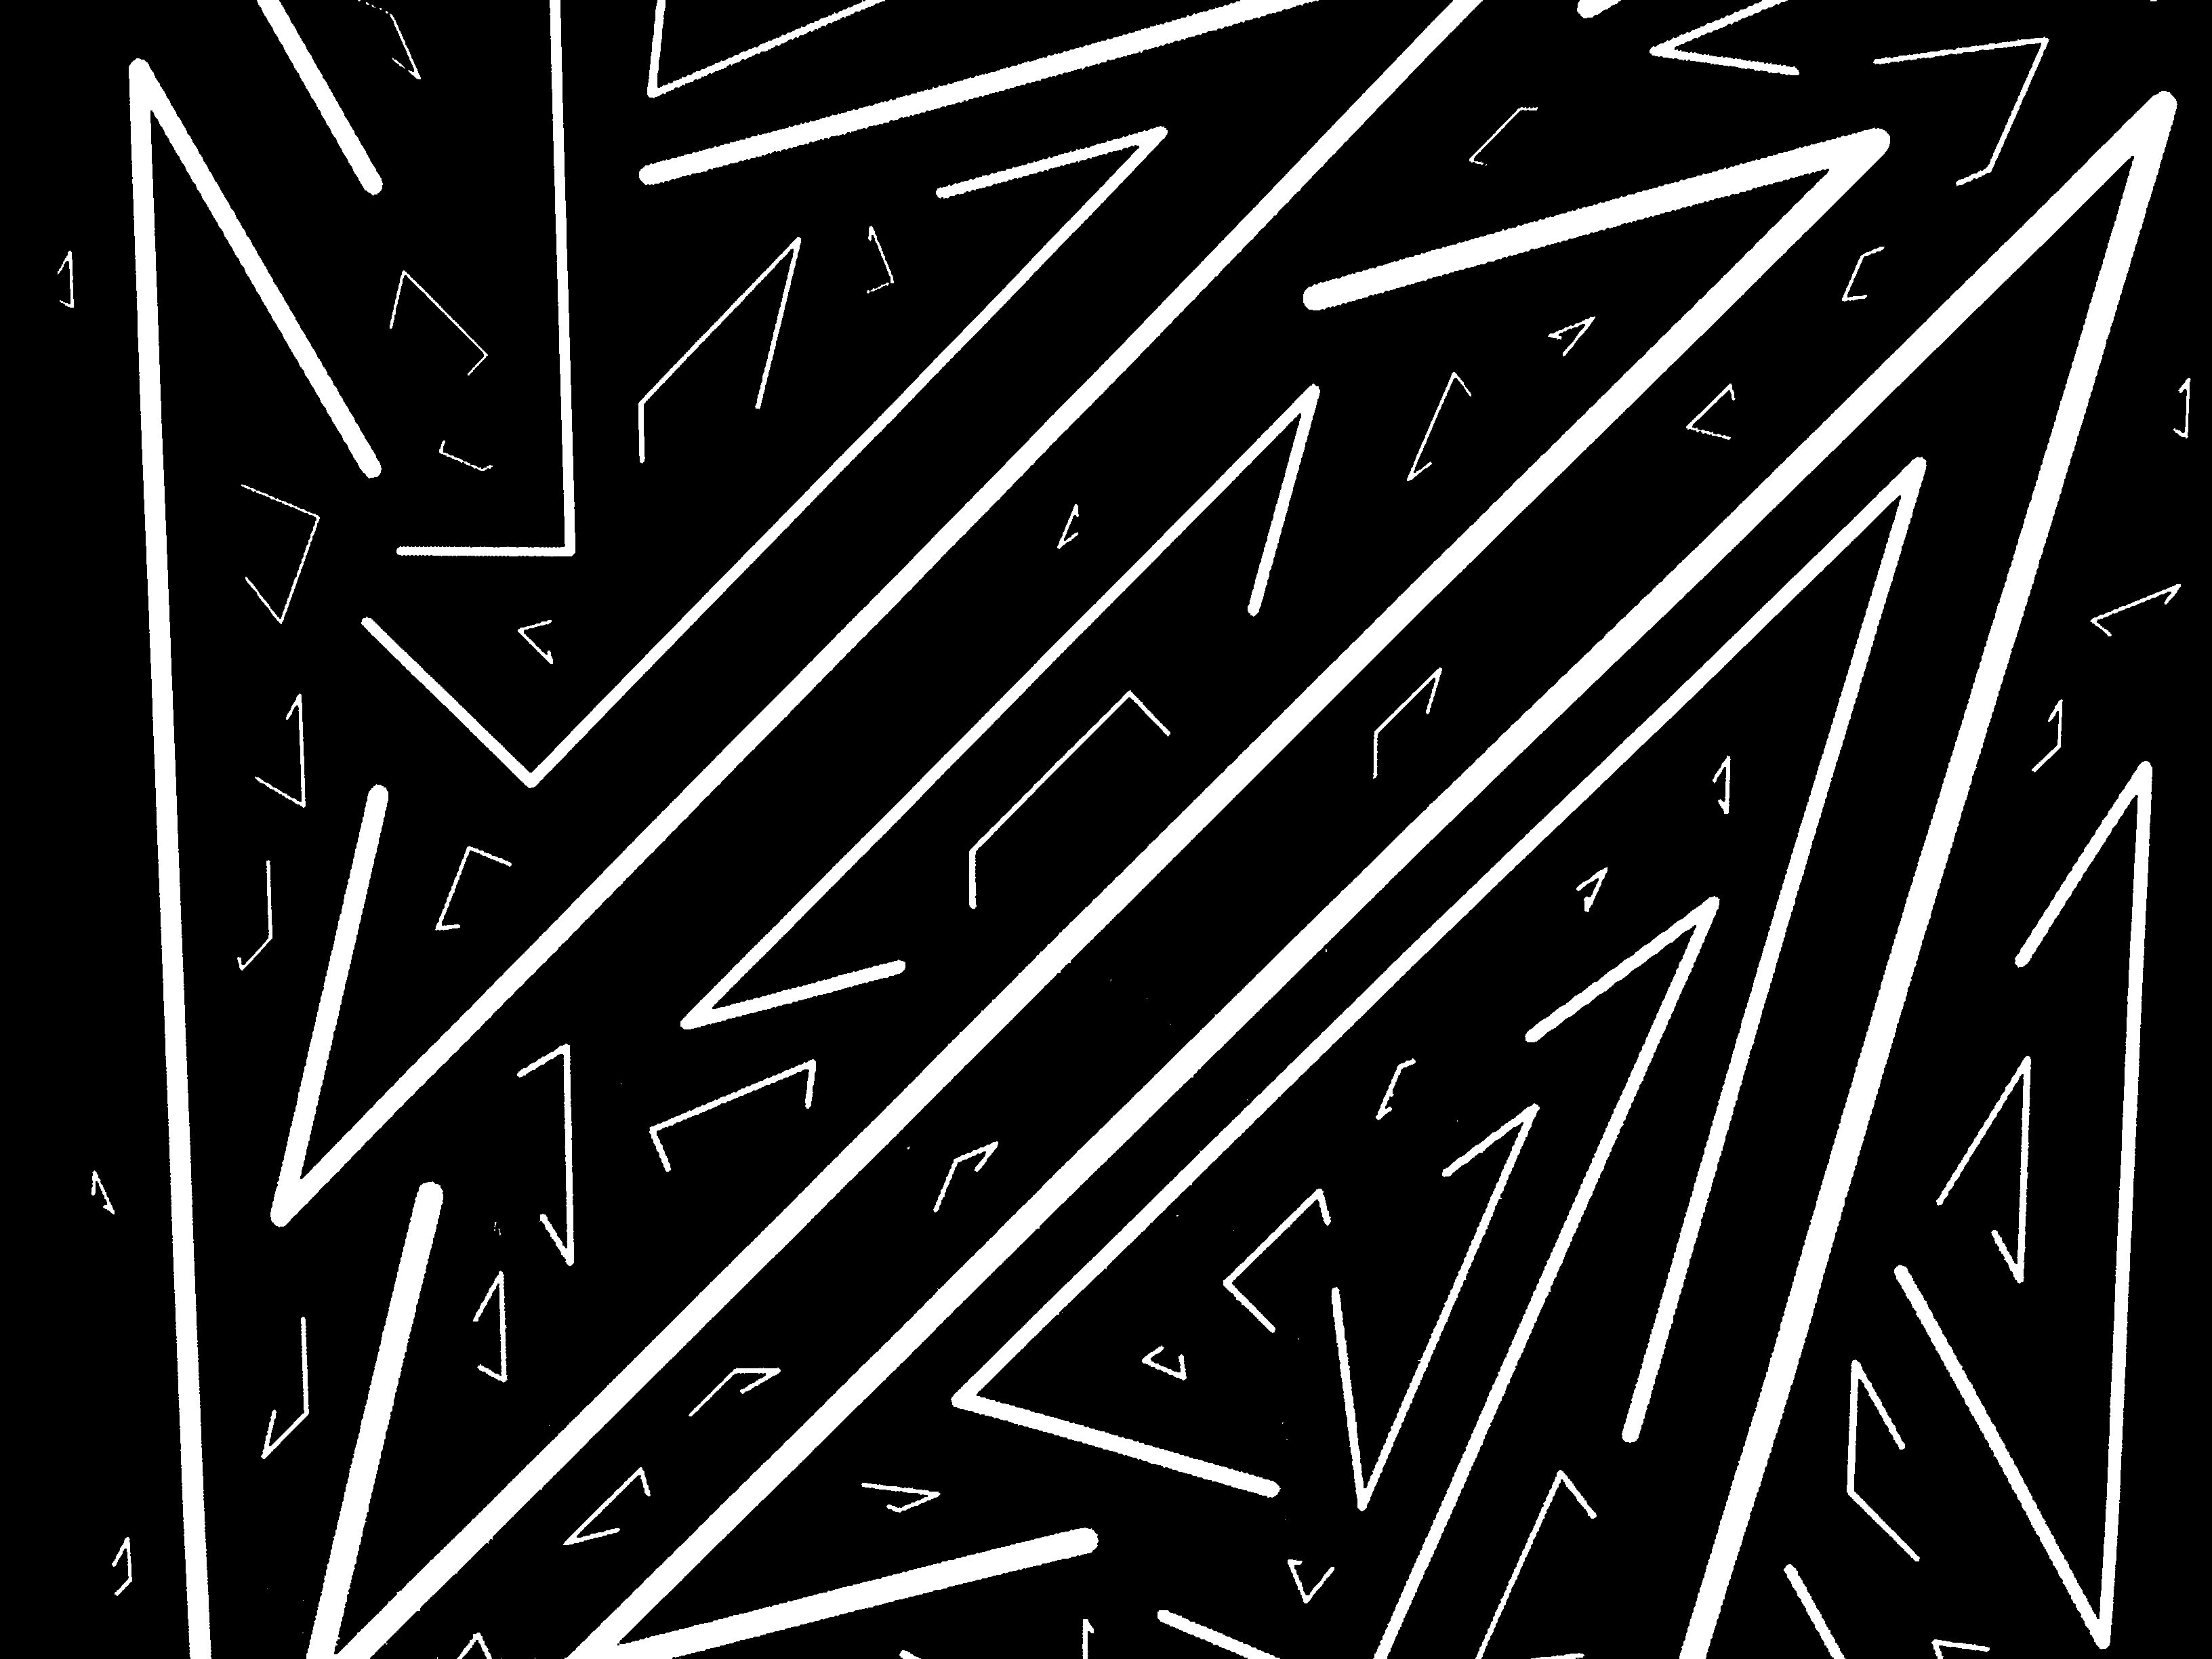
\includegraphics[width=0.9\textwidth]{figures/marker_full_preprocessed.JPG}
	\caption{Marker image after preprocessing}
	\label{fig:markerFullPreproc}
\end{figure}
Figure \figref{markerFullPreproc} shows the output of the preprocessing step of the algorithm.
This is passed to the segmentation logic described in the next section.

%-----------------------------------------------------------------------------------------------
\section{Segmentation}
%-----------------------------------------------------------------------------------------------

The segmentation process is carried out on images roughly like the one shown in figure \figref{markerFullPreproc}.
The segmentation is based on finding continuous contours on the binary image.
The OpenCV framework provides great functionality for this.
The implementation is based on calculating the 8-neighbour chain code for the binary blobs on the image.
The functions returns a list of points for the borders of each distinct contour.
These can be used for calculating the area and circumference of the blobs represented by the contours.

The next step is the filtering of the found blobs.
First, it is necessary to discard the only partially visible and/or unrecognisable quads.
This is done by calculating the bounding box of the contours, and if one of it's sides are touching the image border, the blob is marked as partial.
With this approach it is possible that some fully visible quads that only touch the image border with one of their corner are lost.
This problem can be easily fixed by checking the neighbourhood of the contact point, but this is not yet implemented.

\begin{figure}[ht]
	\begin{subfigure}{0.3\textwidth}
		\centering
		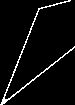
\includegraphics{figures/quad3.png}
	\end{subfigure}
	\begin{subfigure}{0.3\textwidth}
		\centering
		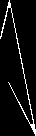
\includegraphics{figures/quad4.png}
	\end{subfigure}
	\begin{subfigure}{0.3\textwidth}
		\centering
		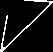
\includegraphics{figures/quad5.png}
	\end{subfigure}
	\caption{Quad candidates after segmentation}
	\label{fig:segmentationOutput}
\end{figure}

The next blob-filtering step is to filter out the false-positive contours.
These false hits can be caused by the light conditions or the scene around the marker.
For this purpose a simple metric is used to measure how likely a blob is to be a quad. 
This metric is the ratio of a blob's area and circumference. 
By experimentation this ratio for quads is found to be in the range of 10 and 50.
The contours with ratios outside these limits are discarded.

The segmentation processes output is available as a singe image with colour-coded\footnote{Gray level, to be exact} blobs or as a list of separate images each containing a quad candidate.
At the current state of the project only the image list representation is used, as te implemented quad detectors take images of single quads as their input.
However, the possibility of implementing detectors to work on whole RQIMs is left open by the colour-coded representation.
Figure \figref{segmentationOutput} shows an example for the output of the segmentation process.

There is also the problem of finding the RQIM on the picture.
This topic was not thoroughly researched in this work, but some basic guidelines were brought up.
The above described segmentation process can be used to identify a marker.
By running the segmentation and filtering process the density of probable quads per image region can be calculated.
On a marker, this should be above the noise level.
By using \textit{a-priori} knowledge of the approximate marker size, the RQIM region on the image can be identified.
When this region is selected, the found probable quads outside it can be discarded.

At this point there is an image or set of images containing potentially good quads.
These are passed as input to the quad detector.
After the quad detection, all image processing tasks are complete.
From then on, only the quad representations are used.

%-----------------------------------------------------------------------------------------------
\section{Pose Calculation}
%-----------------------------------------------------------------------------------------------

The last step of the algorithm is to actually calculate the pose from the detected quads.
According to chapter \sectref{pose}, this is done by using the \textit{robust pose estimation from a planar target} algorithm.
However, the association between the original and the detected quads is not known.
The quad coordinates measured in the previous processing step are of the quads distorted by the projection.
At first, this looks like a deadlock situation: the association of the quads is needed to calculate the camera pose, but without the pose the quads cannot be paired.

To resolve the above issue, an iterative process is proposed.
It is summarised by the following pseudo-code.
The method is a variant of the Random Sample Consensus algorithm.
It's core concept is that randomly selected quad pairs are tested, and the one having the highest number of inliers and least error level is accepted as a solution.
\begin{lstlisting}
find_pose(det_quads, orig_quads):
    threshold = get_thresh(count(det_quads), count(orig_quads))
    pairs = combinations(det_quads, orig_quads)
    pairs.shuffle()
    best_pose = none
    best_error = inf
    for det, orig in pairs:
        pose = robust_planar_pose(det, orig)
        matches = test_pose(pose, det_quads, orig_quads)
        if count(matches) > threshold:
            error = get_detection_error(matches)
            if error < precision:
                return pose
            else if error < best_error:
                best_pose = pose
                best_error = error
    return pose
\end{lstlisting}


